\section{Software Monoliths}\label{section:background:software-monolith}

A monolithic architecture is characterized that there is only one single codebase. Many developers, regardless of which team, are working on the same application. This approach to development was the standard for a very long time and is well supported by various modern development tools. By just having one application, the developers have an overview of the entire application. This software development approach uses a single database with one schema. A prototypical architecture for a monolithic application is shown in Figure \ref{fig:background:monolith:monolith-sketch}.

\ifshowImages
\begin{figure}[H]
  \centering
  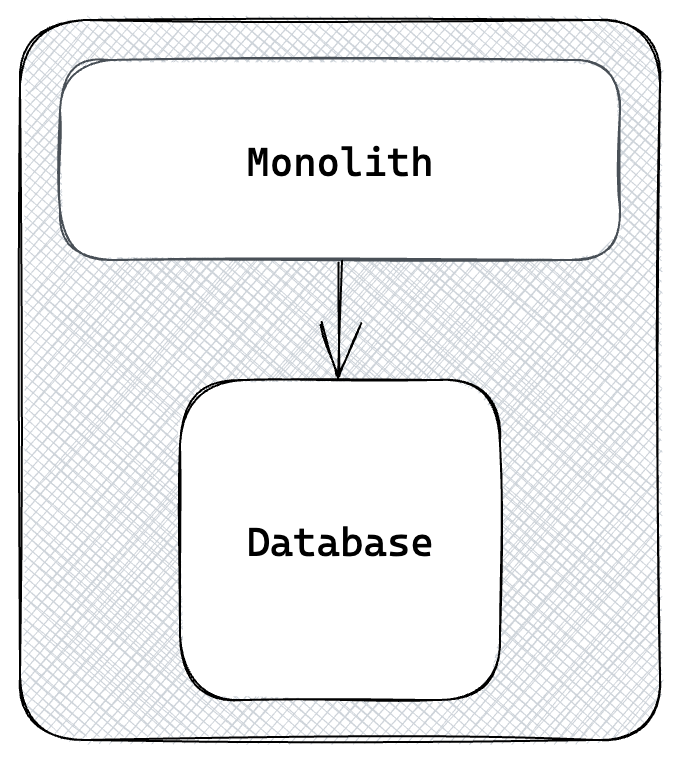
\includegraphics[width=0.3\linewidth]{images/background/monolith/monolith-sketch.png}
  \caption{The typical architecture of a software monolith. (Adapted from \cite[12]{book:2019:newman:background:monolith:monolith-to-microservices})}\label{fig:background:monolith:monolith-sketch}
\end{figure}
\fi

\noindent With a software monolith, applying drastic changes to the complete codebase is easier. Modern \acp{IDE} support for example the refactoring of names, over the complete project. Therefore it is relatively easy to apply changes to every layer of the application, even the database schema. All project parts can be regression tested directly by running the application and the related database. Moreover, the complete application can be built and deployed in one step. Furthermore, it is easy to scale, as multiple instances can be executed behind a load balancer. \cite[4]{book:2018:richardson:background:bff:microservices-patterns}

\bigskip

\noindent If a monolith starts to grow in size, it is essential to have a good software architecture. The code should be put in modules that follow the rules of high cohesion and low coupling of source code. The modularization splits the code into multiple chunks, which are easier to understand however the application is still just a single process. Modules can be developed independently, but the application still has to be deployed as one unit. This approach requires the coordination of various development teams, which could be difficult. \cite[12-13]{book:2018:richardson:background:bff:microservices-patterns} \cite[12-13]{book:2019:newman:background:monolith:monolith-to-microservices} An example of such an architecture is shown in the Figure \ref{fig:background:monolith:module-monolith-sketch}.

\ifshowImages
\begin{figure}[H]
  \centering
  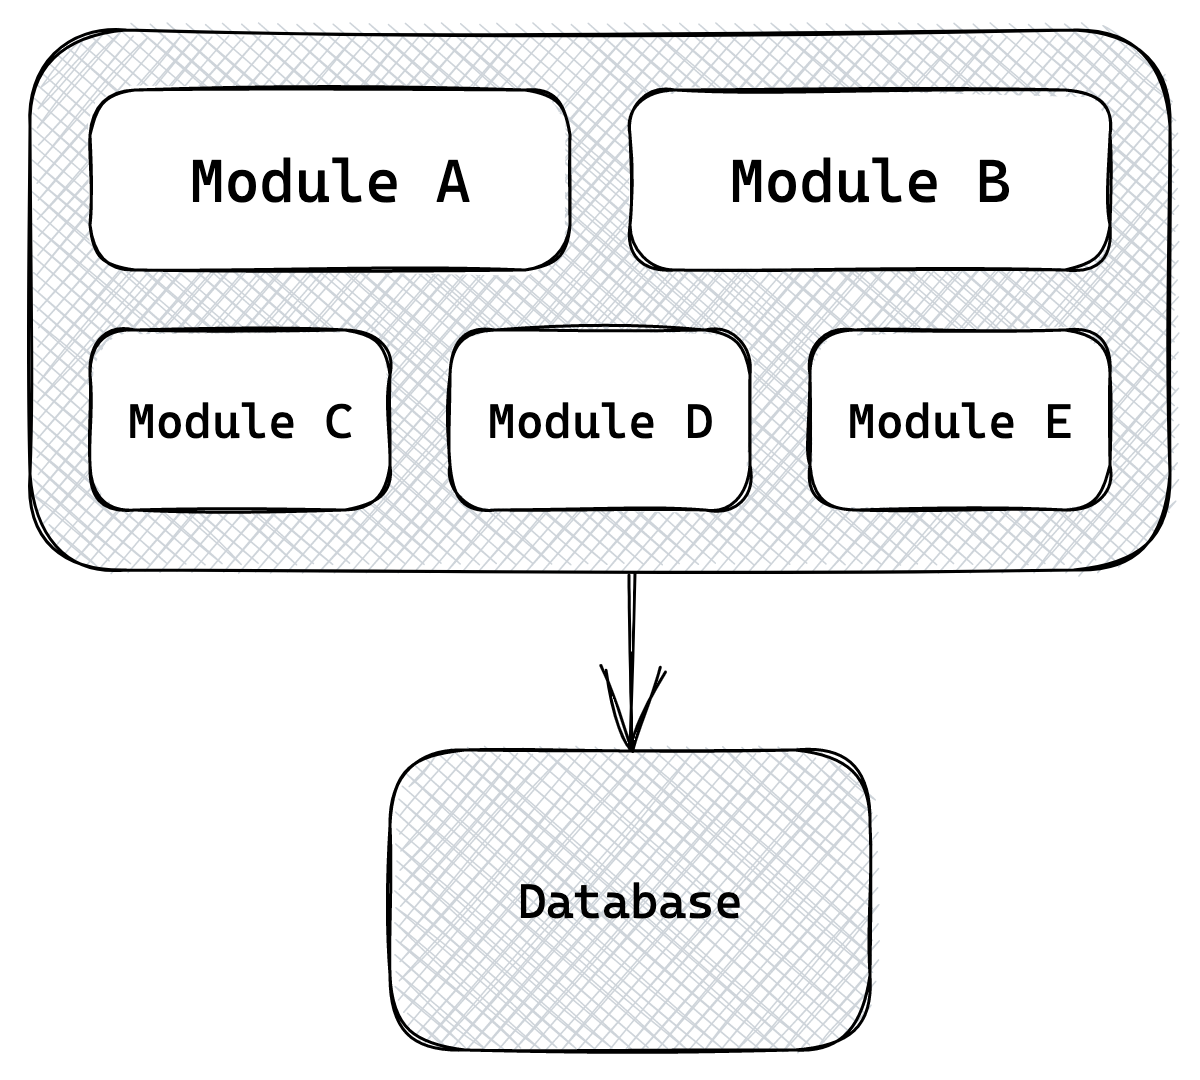
\includegraphics[width=0.3\linewidth]{images/background/monolith/modular-monolith-sketch.png}
  \caption{Structure of a modular monolith. (Adapted from \cite[13]{book:2019:newman:background:monolith:monolith-to-microservices})}\label{fig:background:monolith:module-monolith-sketch}
\end{figure}
\fi

\noindent Modular monoliths provide an excellent choice for many organizations. If there are well-defined module boundaries, parallel working is possible quite easily. However, a database cannot be decomposed into low-coupled modules like with source code. \cite[12-13]{book:2019:newman:background:monolith:monolith-to-microservices}

\subsection{Disadvantages}\label{subsection:background:software-monolith:disadvantages}

With a growing code base, monolithic architectures come with increased complexity. Each new feature adds another complexity level, leading to reduced developer performance. Due to the entry hurdle of understanding the program, developing a new feature might be a time-consuming process. The sheer size of the source code base makes it difficult to comprehend the system because program comprehension is an essential factor in software maintenance. \cite{article:1995:mayrhauser:background:monoliths:program-comprehension-during-software-maintenance-and-evolution} Therefore, developers might create unwanted side effects when fixing a bug. The time for developing a new feature increases drastically, and the internal architecture can also become challenging to understand and maintain. \cite[4-6]{book:2018:richardson:background:bff:microservices-patterns}

\bigskip

\noindent Another problem is that multiple teams might work on the same chunks of code. Two different developers might need to make a change to code in a shared library. A developer may modify the code within a module for which they require additional information. The change might also not be coordinated with other software engineers, which might lead to unexpected behavior in the other developer's code. The circumstance is also known as \textit{confused lines of ownership}, which are frequent sources of errors in a software system. \cite[15]{book:2019:newman:background:monolith:monolith-to-microservices} \cite[7]{inproceedings:2011:bird:background:monoliths:dont-touch-my-code}

\bigskip

\noindent With a monolithic approach, using different technologies is no longer possible, and the technology stack is restricted for the entire lifespan of the monolith. Introducing a different programming language or a different framework is impossible and often leads to a complete rewrite of an application. \cite[6-7]{book:2018:richardson:background:bff:microservices-patterns} The problem with technology is that it always becomes deprecated and obsolete at one point. Applications based on such deprecated technology must be reimplemented with a different programming language or framework. Simply rewriting the application in another framework is not straightforward because the application's functionality must be comprehended.

\subsubsection{Monolithic Systems are not Legacy Systems}\label{subsection:background:software-monolith:not-legacy-systems}

Developing a monolithic application should not be synonymous with writing a legacy application, and the term legacy application should not be used for monolithic systems. \cite[15]{book:2019:newman:background:monolith:monolith-to-microservices} The monolithic architecture is a good starting point for new applications, if some domains of the applications need better understanding and when drastic changes could happen to already implemented features. In the beginning, it is easier to understand the inner workings of the application and make code changes. \cite[43]{book:2019:newman:background:monolith:monolith-to-microservices}
